\subsection{Size and Power with MNIST}
\label{sec:mnist-example}

We use the MNIST handwritten-digit dataset~\citep{lecun2002gradient} as a
high-dimensional, non-Gaussian illustration of two-sample covariance testing.
Each image is represented by $28 \times 28 = 784$ pixel intensities. We combine
the training and test splits, scale pixel intensities to $[0,1]$ using the
dataset loader, and then standardize each pixel separately within the digit-0
and digit-1 samples. Values above 10 after standardization are truncated to
10. This preprocessing focuses the comparison on differences in within-class
correlation structure rather than marginal location and scale.

We compare the Srivastava (2007) and Srivastava--Yanagihara (2014) two-sample
covariance tests. For null calibration, each of 300 replications draws $2N$
distinct digit-0 images without replacement and partitions them into two
nonoverlapping samples of size $N = 200$. For the alternative, one sample of
$N$ digit-0 images and one independently drawn sample of $N$ digit-1 images
are compared. All replications use \code{np.random.default_rng(0)}. The
complete analysis and figure-generation code are provided in
\code{figures/run\_mnist\_example.py}.

\begin{CodeChunk}
\begin{CodeInput}
>>> import numpy as np
>>> from sklearn.preprocessing import StandardScaler
>>> from covtest.datasets import load_mnist
>>> from covtest.methods.hypothesis_two_sample import (
...     srivastava_two_sample_2007,
...     srivastava_yanagihara_two_sample,
... )
>>> N, n_rep = 200, 300
>>> X_tr, y_tr = load_mnist(split="train")
>>> X_te, y_te = load_mnist(split="test")
>>> X = np.concatenate((X_tr, X_te))
>>> y = np.concatenate((y_tr, y_te))
>>> X0 = StandardScaler().fit_transform(X[y == 0])
>>> X1 = StandardScaler().fit_transform(X[y == 1])
>>> X0[X0 > 10] = 10
>>> X1[X1 > 10] = 10
>>> methods = [
...     srivastava_two_sample_2007,
...     srivastava_yanagihara_two_sample,
... ]
>>> rng = np.random.default_rng(0)
>>> null_pvalues = np.empty((n_rep, len(methods)))
>>> alternative_pvalues = np.empty_like(null_pvalues)
>>> for i in range(n_rep):
...     idx0 = rng.choice(X0.shape[0], size=2 * N, replace=False)
...     idx1 = rng.choice(X1.shape[0], size=N, replace=False)
...     for j, method in enumerate(methods):
...         null_pvalues[i, j] = method(X0[idx0[:N]], X0[idx0[N:]])["p_value"]
...         alternative_pvalues[i, j] = method(X0[idx0[:N]], X1[idx1])["p_value"]
\end{CodeInput}
\end{CodeChunk}

Figure~\ref{fig:mnist} summarizes the input distributions, null calibration,
and empirical rejection rates at $\alpha = 0.05$. The pixel-intensity
distributions are strongly non-Gaussian, with substantial mass near zero and a
right-skewed positive tail. Under the digit-0 versus digit-0 null, the
empirical rejection rates are 0.023 for Srivastava (2007) and 0.003 for
Srivastava--Yanagihara (2014). Thus, both procedures are conservative in this
non-Gaussian design, particularly the latter. Under the digit-0 versus
digit-1 comparison, the corresponding empirical rejection rates are 0.687 and
1.000. These results illustrate that the two methods can detect marked
differences in the covariance structure of the two digit classes, while also
showing the importance of checking null calibration when applying large-sample
procedures to structured, non-Gaussian image data.

\begin{figure}[t!]
\centering
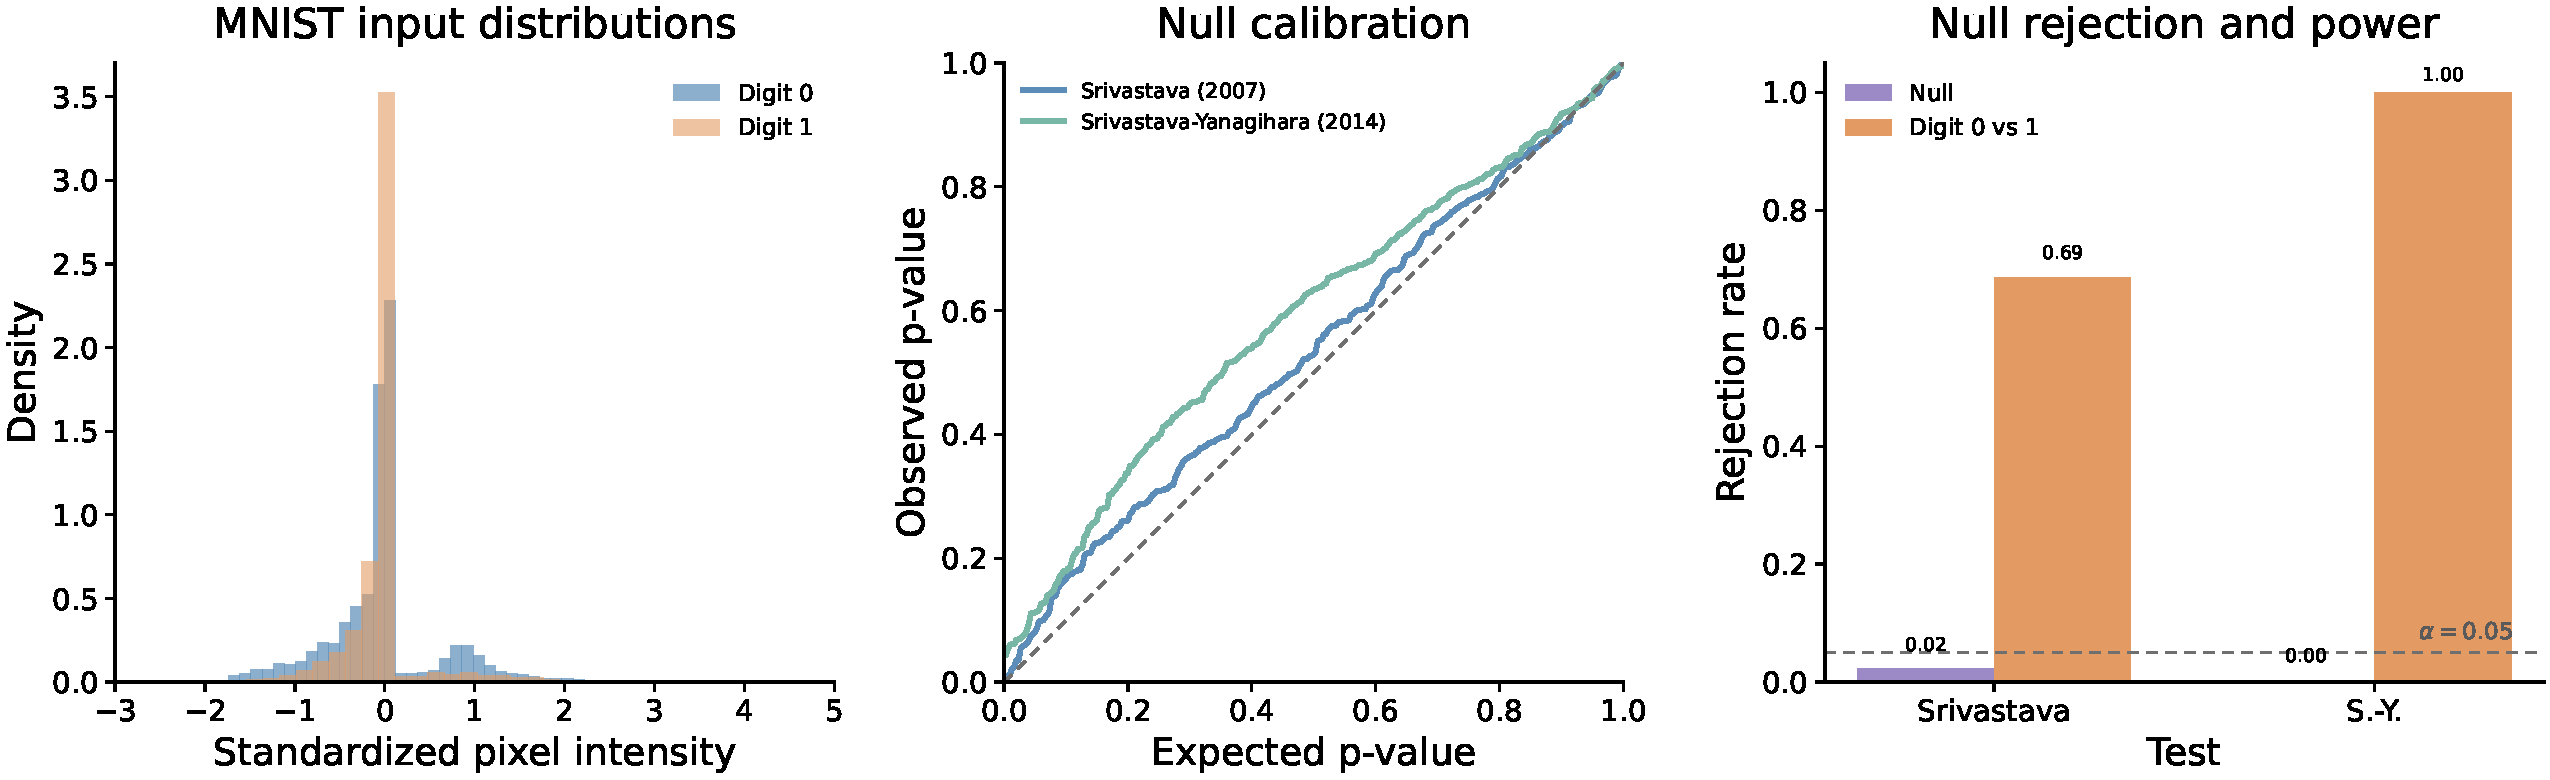
\includegraphics[width=\textwidth]{figures/figure_mnist.pdf}
\caption{\label{fig:mnist} MNIST two-sample covariance-test results for
digit 0 versus digit 1. The left panel shows the standardized pixel-intensity
distributions. The middle panel presents P--P plots for the digit-0 versus
digit-0 null comparison. The right panel reports empirical rejection rates at
$\alpha = 0.05$ under the null and under the digit-0 versus digit-1
alternative, based on 300 replications with $N = 200$ observations per group.}
\end{figure}

\subsection{Multiple Hypothesis Testing with TCGA}
\label{sec:tcga-example}

In our second example, we demonstrate how \pkg{scikit-covtest} combines
two-sample covariance-structure tests with multiple-testing procedures. We use
the gene-expression cancer RNA-Seq dataset~\citep{fiorini2016gene}, a random
extraction from the RNA-Seq (HiSeq) PANCAN dataset assembled by The Cancer
Genome Atlas Pan-Cancer Analysis Project~\citep{weinstein2013cancer}. The
dataset contains 801 samples and 20,531 gene-expression features. We compare
breast invasive carcinoma (BRCA, $n = 300$) with lung adenocarcinoma (LUAD,
$n = 141$).

To target differences in correlation rather than marginal variances, we
standardize every expression feature separately within BRCA and LUAD. We then
partition the 20,531 features into 4,106 nonoverlapping blocks of five
consecutive features, discarding the final trailing feature. The first column
returned by \code{load_tcga()} is a sample identifier and is removed before
the expression matrix is converted to numeric form.

The Srivastava (2007) statistic is undefined for blocks whose pooled
trace-square covariance estimate is zero. Of the 4,106 initial blocks, 30 are
degenerate in this sense and are excluded before multiplicity correction. The
remaining 4,076 valid block-level $p$-values form the family used for the
Bonferroni, Benjamini--Hochberg (BH), and Benjamini--Yekutieli (BY)
adjustments. The complete analysis and figure-generation code are provided in
\code{figures/run\_tcga\_example.py}.

\begin{CodeChunk}
\begin{CodeInput}
>>> import numpy as np
>>> from sklearn.preprocessing import StandardScaler
>>> from covtest.datasets import load_tcga
>>> from covtest.methods.hypothesis_two_sample import srivastava_two_sample_2007
>>> from covtest.multiplicity.fdr import benjamini_hochberg, benjamini_yekutieli
>>> from covtest.multiplicity.fwer import bonferroni
>>> X_raw, y = load_tcga()
>>> X = X_raw[:, 1:].astype(float)  # Drop the sample-ID column.
>>> X_brca = StandardScaler().fit_transform(X[y == "BRCA"])
>>> X_luad = StandardScaler().fit_transform(X[y == "LUAD"])
>>> n_groups = X.shape[1] // 5
>>> pvalues = np.full(n_groups, np.nan)
>>> for i in range(n_groups):
...     idx = 5 * i + np.arange(5)
...     try:
...         pvalues[i] = srivastava_two_sample_2007(
...             X_brca[:, idx], X_luad[:, idx]
...         )["p_value"]
...     except ValueError:
...         pass  # Degenerate block; exclude before multiplicity correction.
>>> valid = np.isfinite(pvalues)
>>> tested_pvalues = pvalues[valid]
>>> bonf = bonferroni(tested_pvalues)
>>> res_bh = benjamini_hochberg(tested_pvalues)
>>> res_by = benjamini_yekutieli(tested_pvalues)
\end{CodeInput}
\end{CodeChunk}

At $\alpha = 0.05$, Bonferroni rejects 23 of the 4,076 valid blocks. BH
rejects 41 blocks, whereas the more conservative BY procedure rejects 26
blocks. The ordering $23 \leq 26 \leq 41$ is expected: Bonferroni controls
the family-wise error rate, whereas BH and BY control the false discovery
rate, with BY additionally accounting for arbitrary dependence through its
harmonic correction. Figure~\ref{fig:tcga} displays the block-level p-values
and the BH and BY adjusted p-values. Values with $-\log_{10}$ adjusted
$p$-values at or above 20 are displayed at 20 to avoid numerical underflow
dominating the plot.

\begin{figure}[t!]
\centering
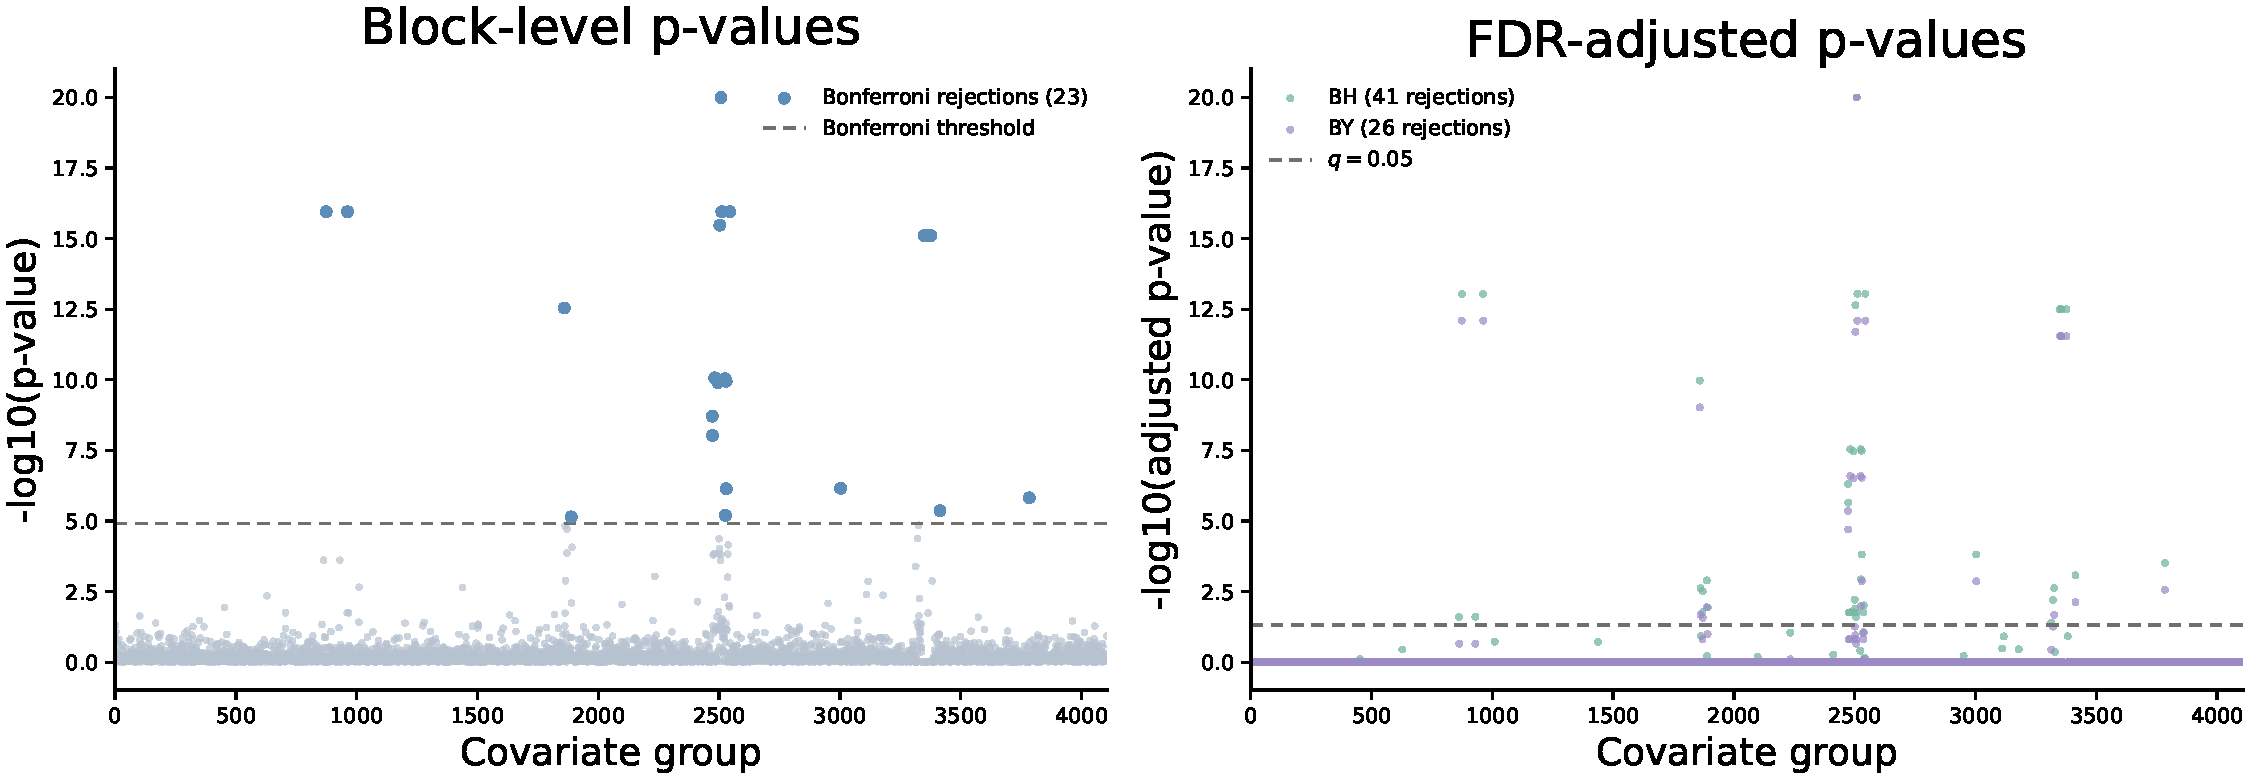
\includegraphics[width=\textwidth]{figures/figure_tcga.pdf}
\caption{\label{fig:tcga} TCGA results for the BRCA-versus-LUAD comparison.
The left panel shows block-level $p$-values for the 4,076 valid five-feature
blocks; the dashed line denotes the Bonferroni threshold at $\alpha = 0.05$,
and highlighted points are Bonferroni rejections. The right panel shows BH and
BY adjusted $p$-values. Thirty degenerate blocks were excluded before
multiplicity correction.}
\end{figure}
